%Capítulo 3

\section{Diseño del Estudio}
    
    \textbf{\textit{Descripción}}
    
    Describe con claridad el método que se va a aplicar al tipo de investigación y las razones de su elección.
    \begin{itemize}
        \item Acción del investigador sobre las variables.
        \item Cinética del estudio.
    \end{itemize}
    
    \textbf{\textit{Criterios de calidad}}
    
    La metodología responde a la pregunta: \textbf{¿Cómo se elaborará la investigación?}
    El diseño se debe de realizar en función del grado de validez y generalización que se pretende dar al proyecto de investigación, tomando en cuenta:
    
    \begin{itemize}
        \item Grado de confiabilidad
        \item Control de sesgo
        \item Tamaño de la muestra
        \item Control o eliminación de variables extrañas
        \item Grado o nivel de confiabilidad de los instrumentos
    \end{itemize}
    
    Es siguiente es un ejemplo usando Tikz. Llama Figura \ref{fig:ArregloFuentes}
    
    \begin{figure}
        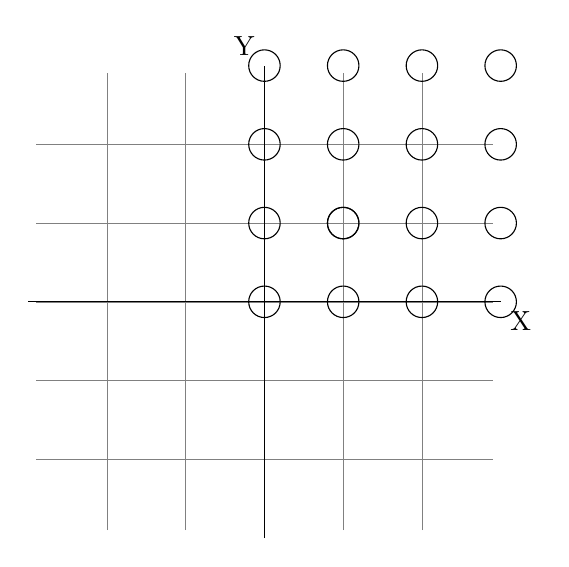
\begin{tikzpicture}
            \draw[step=1cm,gray,very thin] (-2.9,-2.9) grid (2.9,2.9);
            % Draw X axis
            \draw (-3,0) -- (3,0) node[anchor=north west] {X};
            % Draw Y axis
            \draw (0,-3) -- (0,3) node[anchor=south east] {Y};
            %+X +Y
            \draw (0,0) circle (0.2);
            \draw (1,0) circle (0.2);
            \draw (2,0) circle (0.2);
            \draw (3,0) circle (0.2);
            \draw (1,1) circle (0.2);
            \draw (0,1) circle (0.2);
            \draw (0,2) circle (0.2);
            \draw (0,3) circle (0.2);
            \draw (1,1) circle (0.2);
            \draw (1,2) circle (0.2);
            \draw (1,3) circle (0.2);
            \draw (2,1) circle (0.2);
            \draw (2,2) circle (0.2);
            \draw (2,3) circle (0.2);
            \draw (3,1) circle (0.2);
            \draw (3,2) circle (0.2);
            \draw (3,3) circle (0.2);  
        \end{tikzpicture}
        \centering
        \caption{La figura es un ejemplo.}
        \label{fig:ArregloFuentes}
    \end{figure}


\section{Universo de trabajo y muestra}

    \textbf{\textit{Descripción}}
    
    Describe la población con la que se trabajará en la investigación, y el procedimiento para la selección de la muestra.
    
    \textbf{\textit{Criterios de calidad}}
    
    El tamaño de la muestra deberá corresponder al nivel de confiabilidad deseado y pertinente al estudio.

\section{Operacionalización de variables}

    \textbf{\textit{Descripción}}
    
    Es llevar una variable de un nivel abstracto a un nivel concreto; es decir, que permita medirla o calificarla. En esta sección, por cada variable incluida en el estudio, se deberá indicar:
    
    \begin{itemize}
        \item Definición teórica.
        \item Definición operacional y, en su caso, criterios diagnósticos.
        \item Nivel de medición.
        \item Indicadores.
        \item Ítems de los instrumentos de investigación respectivos.
    \end{itemize}
    
    \textbf{\textit{Criterios de calidad}}
    
    Debe de contener una definición conceptual previa por cada variable del estudio y su desarrollo descriptivo de cómo se operativizó.

\section{Instrumentos de Investigación}

    \textbf{\textit{Descripción}}
    
    Detalla los elementos y tipos de instrumentos que se emplearán, y se justifica su uso \cite{latexcompanion}.
    En algunas ocasiones, se deberá diseñar los instrumentos, lo cual implica un sub-proyecto de investigación dentro de la investigación.
    
    \textbf{\textit{Criterios de calidad}}
    
    Validez y confiabilidad demostrada.

\section{Diseño Técnico y metodológico para la obtención y análisis de la información}

    \textbf{\textit{Descripción}}
    
    Se especifica el diseño de la investigación y se da una descripción técnica y metodológica de cómo se realizó el análisis de los datos.
    Se mencionan las pruebas estadísticas empleadas y/o el programa de cómputo utilizado en el análisis de los datos.
    
    \textbf{\textit{Criterios de calidad}}
    
    Debe explicar de forma ordenada el proceso que se realizó para lograr el objetivo de la investigación.
    Deben indicarse las técnicas de análisis, el grado y nivel de confiabilidad de las pruebas que se emplearon.